%----------------------------------------------------------------------------------------
%	PACKAGES AND THEMES
%----------------------------------------------------------------------------------------
\documentclass[aspectratio=169,xcolor=dvipsnames]{beamer}
\usetheme{SimplePlusAIC}

\usepackage{hyperref}
\usepackage{graphicx} % Allows including images
\usepackage{booktabs} % Allows the use of \toprule, \midrule and  \bottomrule in tables
\usepackage{svg} %allows using svg figures
\usepackage{tikz}
\usepackage{makecell}
\graphicspath{ {./images/} }
\usepackage{amsmath}
\usepackage{amssymb}
\newcommand*{\defeq}{\stackrel{\text{def}}{=}}

%----------------------------------------------------------------------------------------
%	TITLE PAGE
%----------------------------------------------------------------------------------------

\Huge\title{Cubical Set} % The short title appears at the bottom of every slide, the full title is only on the title page
\subtitle{Honours Research Presentation}
\author[Wang]{Ziang Wang}
% Your institution as it will appear on the bottom of every slide, maybe shorthand to save space


\raggedright\date{\today} % Date, can be changed to a custom date
%----------------------------------------------------------------------------------------
%	PRESENTATION SLIDES
%----------------------------------------------------------------------------------------

\begin{document}

\begin{frame}[plain]
    % Print the title page as the first slide
    \titlepage
\end{frame}
%------------------------------------------------
\begin{frame}{Introduction}
    \begin{definition}
        Elementary interval: \\
        If $l \in \mathbb{R}$, a closed interval in $\mathbb{R}$ that has the form of \texttt{I} $ = [ l,l+1 ]$ or $[ l ]$ is called elementary interval.
    \end{definition}
\begin{itemize}
        \item  $[ l,l+1 ]$ is called non degenerated component 
        \item  $[ l ]$ is called degenerated component 
    \end{itemize}
    
\end{frame}

%------------------------------------------------
\begin{frame}{Introduction}
    \begin{definition}
        Elementary Cube: \\
        If Q is a finite product of elementary intervals, namely, \\
                     \begin{center}
                          $Q =$ \texttt{I_1} $\times$\texttt{I_2} $\times$\texttt{I_3} $...$ $\times$\texttt{I_d}, \\
                     \end{center} 
        \textsf{Q is then an elementary cube.}
    \end{definition}

    \begin{itemize}
        \item $d$ is called the embedding number. $emb(Q) = d$
        \item The dimension of Q is the number of non degenerated components in Q.
        \item $K^d_n$ means the collection that contains every elementary cubes in a space that has the dimension n and embedding number d.
    \end{itemize}
    
\end{frame}

%------------------------------------------------
\begin{frame}{Introduction}
    \begin{definition}
        K-chain:  \\
        K-chain is the sum of the span of numerous elementary cubes. \\
        Or, 
        let $\alpha_1, \alpha_2 ...$ be every $\mathbb{R}$, k-chain for $Q_1, Q_2 ...$ is \\
        $$C = \sum \alpha_i \cdot \widehat{Q_i}$$
        
    \end{definition}

\end{frame}
%------------------------------------------------
\begin{frame}{Method}
    \begin{itemize}
        \item Find the product of k-chains  \\[10pt]

        \item Find the boundary operator of k-chain
    \end{itemize}
\end{frame}

%------------------------------------------------

\begin{frame}{Method}
From intuition, what would the product between these two spaces be? \\
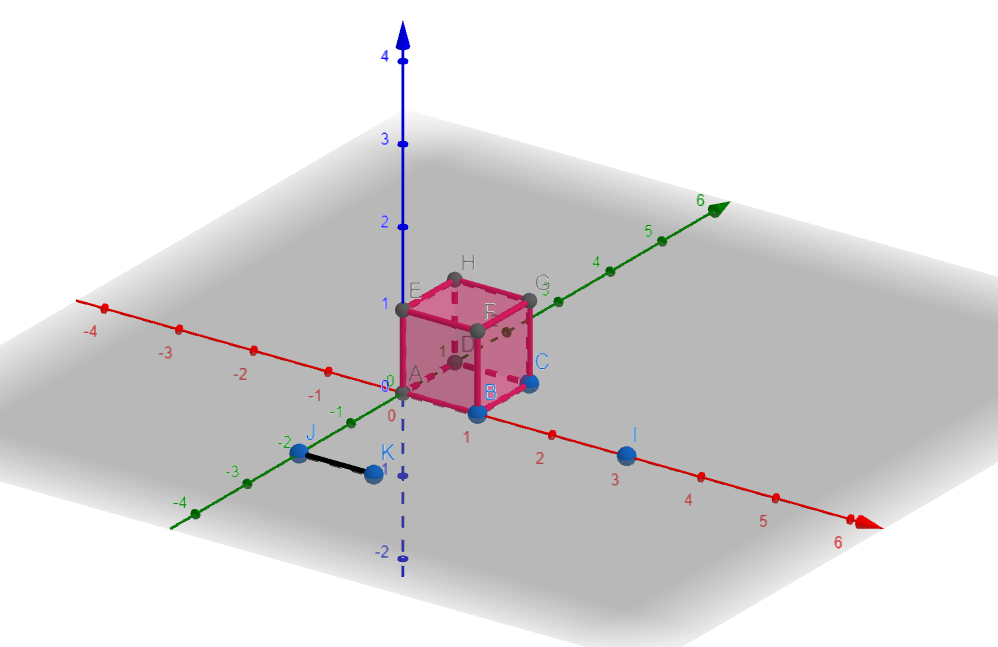
\includegraphics[scale=0.2]{1}     $C_1 = \alpha_1 \cdot \widehat{[0,1] \times [0,1] \times [0,1]} + \alpha_2 \cdot \widehat{[0,1] \times [-2]} + \alpha_3 \cdot \widehat{[3]} $
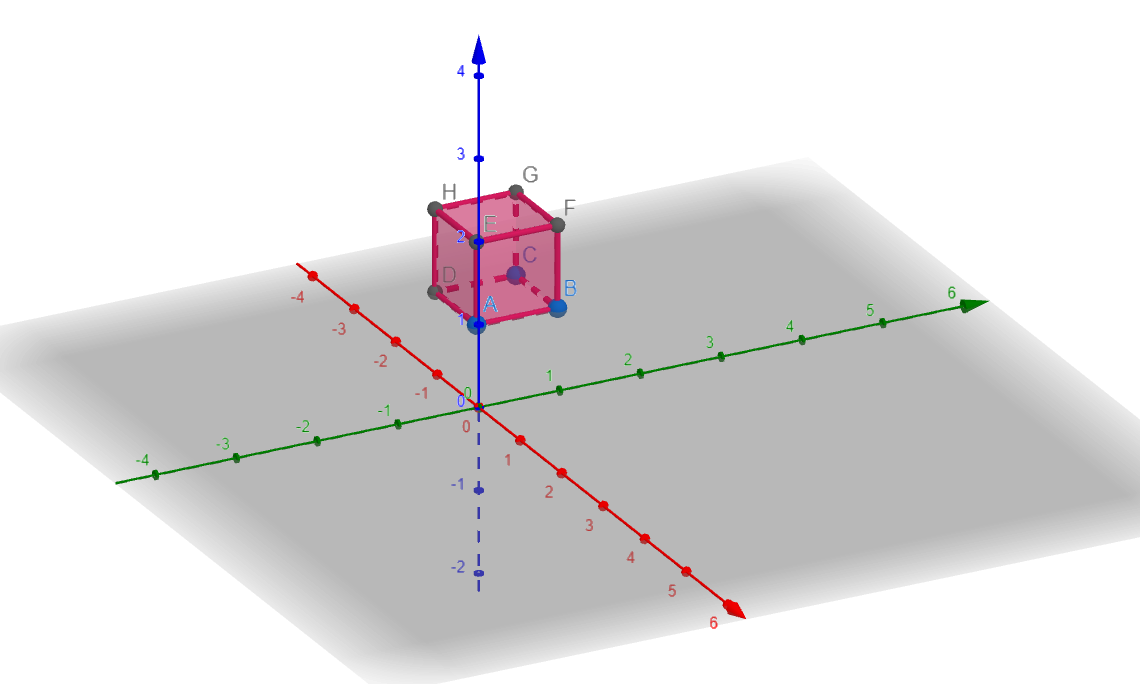
\includegraphics[scale=0.2]{2}     $C_2 = \alpha_4 \cdot \widehat{[-1,0] \times [0,1] \times [1,2]}$  


\end{frame}

%------------------------------------------------

\begin{frame}{Method}
Inspired by box product, it should be the sum of every combination between the elementary cubes of two chains, so
    \begin{function}
        $$C_1 \times C_2 = \sum \alpha_i \cdot \alpha_j \textbf{ }\widehat{Q_i \times Q_j}$$
    \end{function}
\end{frame}

%------------------------------------------------

\begin{frame}{Method}
    Let $c_1 \text{ induced by } K_K$ and $c_2 \text{ induced by } K'_K$. Cubical product is defined as
$$c_1 \diamond c_2 = \sum_{p\in K_K,Q \in K'_K}<c_1, \widehat{P}><c_2, \widehat{Q}> \widehat{P \times Q}$$
where, \\
$$<c_1,c_2>=\sum \alpha_i \beta_i$$
\end{frame}

%------------------------------------------------

\begin{frame}{Method}
Now, for boundary. To find boundary generally, we want an operator($\partial_s$) that input a Q with dimension $s$ and return a Q' that has dimension $s-1$. \\[10pt]
Some facts we know are: \\
\begin{itemize}
    \item   \begin{align*}
        \partial_1\colon  [l,l+1] &\mapsto [l+1] - [l]\\
                         [l] &\mapsto 0 
            \end{align*}
    \item For Q that $dim(Q)>1$, its each non degenerated interval will undergo $\partial_1$, degenerated interval will simply disappear. 
    \item The operator needs to have an order.
\end{itemize}
\end{frame}

%------------------------------------------------
\begin{frame}{Method}
e.g
\\[10pt]
A simple cube of $[0,1] \times [0,1] \times [0,1]$ will become $(A_4-A_6) + (A_5-A_3) + (A_2-A_1)$

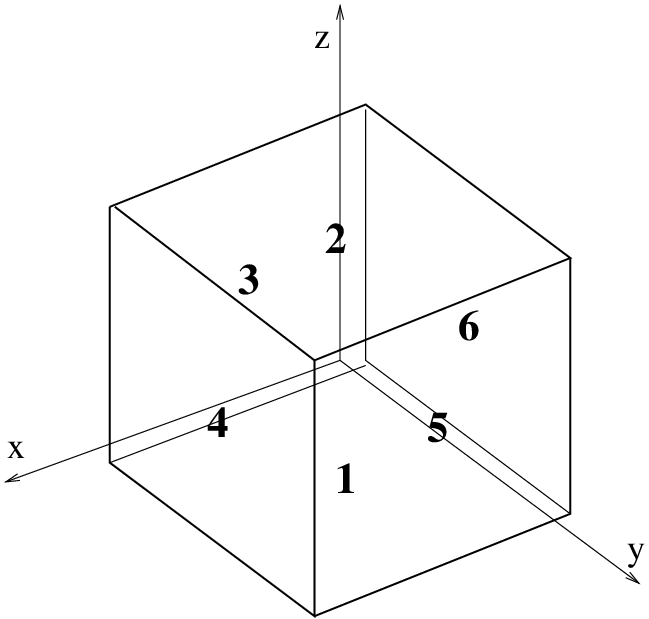
\includegraphics[width=0.25\textwidth]{3}

\end{frame}

%------------------------------------------------
\begin{frame}{Conclusion}
Recursively defined,
    $$\partial_k \colon K^d_k \longrightarrow K^d_{k-1}$$
For $d>1$ let $I = I_1(Q)$, $P= I_2(Q) \times ... \times I_d(Q)$
$$\partial_k \widehat{Q}\text{ } =\text{ } \partial_k_1 \text{ } \widehat{I} \diamond \widehat{P} + (-1)^{k_1} \text{ }\widehat{I} \diamond \partial_k_2 \widehat{P}$$
where $k_1 = dim(I)$, $k_2=dim(P)$ \\
\\[10pt]
Absolutely defined, let $\{U_1,U_2 ...\}$ be the non degenerated interval, it is mixed with many degenerated ones\\
$$\partial \widehat{Q}\text{ } =\text{ } \sum \pm \partial \widehat{U_i} \diamond \{\widehat{Q_U_i}\} $$
where $\widehat{Q_U_i}$ is the interval list after $\widehat{U_i}$
\end{frame}


%------------------------------------------------


\begin{frame}{References}
    % Beamer does not support BibTeX so references must be inserted manually as below
    \footnotesize{
        \begin{thebibliography}{99}
            \bibitem[, 2004]{} Kaczynski Mischaikow Mrozek (2004)
            \newblock Computational Homology, Springer New York, NY. Published: 01 December 2010
        \end{thebibliography}
    }
\end{frame}
%------------------------------------------------


\end{document}